\clearpage
\chapter{Mastery Workbook 10}

% Chapter page
\section{Probability Workbook}

\horizontalline{0}{0}

\begin{center}
    \Large{\textbf{I have neither given nor received unauthorized assistance.}}
    \horizontalline{0}{0}
    \large{\textbf{Taylor James Larrechea}}
    \horizontalline{0}{0}
\end{center}

% Problem 1
\begin{problem}{Problem 1}
    \begin{statement}{Problem Statement}
        Section 7.1 Do \# 39, page 452. Do not use the argument from the back of the book for this. Explain COMPLETELY in your own words.

        \subsection*{Original Question:}

        Explain what is wrong with the statement that in the Monty Hall Three-Door Puzzle the probability that the prize is behind the first door you select and the probability that the prize is behind 
        the other of the two doors that Monty does not open are both 1/2, because there are two doors left.
    \end{statement}

    \begin{Highlight}[Solution]
        At the beginning of the problem, there is a 1/3 probability that you correctly select the door that has the prize behind it. This means that there is a 2/3 probability that you did not select the
        correct door with the prize behind it.

        When Monty goes to open up a door that he knows does not have the prize behind it, there remains only two doors that are left in the game. One would incorrectly think at this point that the probability
        is 1/2 because there are two doors left. This is incorrect because \textbf{it is not incorporating the original probability at the beginning of the game}.

        If we were to simulate this game say 100 times, the probabilities mean that we would have correctly selected the door at the beginning 33 times and the other 67 times the prize would be behind 
        one of the other two doors. So regardless, this does not equate to a 1/2 in probability even though there are only two doors left.
    \end{Highlight}
\end{problem}

% Problem 2
\begin{problem}{Problem 2}
    \begin{statement}{Problem Statement}
        Pg. 452 Do \# 40, page 452. Show you work and explain. ALL PARTS.

        \subsection*{Original Question:}

        Suppose that instead of three doors, there are four doors in the Monty Hall puzzle. What is the probability that you win by not changing once the host, who knows what is behind each door, opens 
        a losing door and gives you the chance to change doors? What is the probability that you win by changing the door you select to one of the two remaining doors among the three that you did not select?
    \end{statement}

    \begin{Highlight}[Solution]
        At the beginning of this game, there is a 1/4 probability that you correctly choose the door that has the prize behind it. This means that there is a 3/4 probability that you did not correctly choose
        the door with the prize behind it.

        \subsubsection*{Not Changing Doors:}

        In this scenario we are not changing our original choice. This means that the probability of us winning with not changing doors is still 
        
        \setcounter{equation}{0}
        \begin{equation}
            \mathbf{1/4} \text{ or } \mathbf{25\%}.
        \end{equation}

        \subsubsection*{Changing Doors:}

        In this scenario we are going to switch our door with one of the remaining two doors that have not been opened. Originally, we had a 3/4 probability that we did not correctly choose the door 
        with the prize. After Monty opens a door that does not have the prize behind it, the 75\% probability of the prize lying behind one of the unopened doors is split between the remaining two
        doors that we have to choose from.

        This means that the 75\% (or 3/4) probability is split between the remaining two doors. So, if we switch between one of the remaining two doors we will have a probability of winning of

        \begin{equation}
            \frac{1}{2} \cdot \frac{3}{4} = \mathbf{3/8} \text{ or } \mathbf{37.5 \%}.
        \end{equation}
    \end{Highlight}
\end{problem}

% Problem 3
\begin{problem}{Problem 3}
    \begin{statement}{Problem Statement}
        Section 7.3 Do \# 10, page 476. Show all work and explain. (use \# 9 as warm up).
    \end{statement}
\end{problem}

% Problem 4
\begin{problem}{Problem 4}
    \begin{statement}{Problem Statement}
        Grading only (a) and (b). \textbf{Show all work} and explain, see related video (Probability Theory 2 time 11:00) and assumptions. \vspace*{1em}

        Suppose a six-sided die is loaded so that:

        \begin{itemize}
            \item 1,3,4 and 6 come up equally often.
            \item 2 comes up as 3 times often as 3.
            \item 5 comes up as twice as often as 6.
        \end{itemize}

        \begin{enumerate}[label = (\alph*)]
            \item Find the probability distribution of this die.
            \item What is the probability that you roll an odd number with this die?
            \item What is the probability that you roll the die twice in a row, and the 2 rolls sum to 7?
            \item What is the probability that you roll the die twice in a row and the 2 rolls sum to 7 GIVEN the first roll is an even number? (see Piazza for important hint)
            \item Based on your answers, to a and b, are these 2 events independent? Explain.
        \end{enumerate}
    \end{statement}

    \begin{Highlight}[Solution - Part (a)]
        We know that if we sum up all of the probabilities of this die they must add up to 1. Since this is a six sided die, we know that there are only six possibilities for what can be rolled regardless
        of the weighting of each probability.

        We can represent this mathematically where $x$ is the probability of one side showing up. Taking into account the information that was given to us our equation for the probabilities of each side
        are

        \setcounter{equation}{0}
        \begin{equation}
            x + 3x + x + x + 2x + x = 9x = 1 \hspace*{10pt} \rightarrow \hspace*{10pt} x = \frac{1}{9}.
        \end{equation}
        Now, taking into account the weighting of each side we can then say
        \begin{align}
            \text{Sides: } & 1,3,4,6 & \text{Probability} =  \frac{4}{9} \\
            \text{Side: } & 2 & \text{Probability} =  \frac{3}{9} = \frac{1}{3} \\
            \text{Side: } & 5 & \text{Probability} =  \frac{2}{9}.
        \end{align}
        The probability of a 1,3,4 or 6 showing up is $\frac{1}{9}$ each.
    \end{Highlight}

    \begin{Highlight}[Solution - Part (b)]
        We know that the probability of a 1 or 3 being rolled is $\frac{1}{9}$ each. The probability of a 5 being rolled is $\frac{2}{9}$. To find the probability of rolling an odd number, we need to 
        sum the probabilities of rolling a 1, 3, or 5. Namely

        \begin{equation}
            \mathcal{P}(1) + \mathcal{P}(3) + \mathcal{P}(5) = \frac{1}{9} + \frac{1}{9} + \frac{2}{9} = \frac{4}{9}.
        \end{equation}
        Therefore the probability of rolling an odd number is then $\frac{4}{9}$.
    \end{Highlight}
\end{problem}

% Problem 5
\begin{problem}{Problem 5}
    \begin{statement}{Problem Statement}
        Read Section 7.4 pp. 477-479.

        \begin{itemize}
            \item Define `Expected Value' in your own words.
            \item Redo example 3 p. 479, and find the expected value of a SINGLE die.
            \item What is surprising (or maybe confusing) about this answer?
            \item What does it mean if the expected value is NOT a value that can actually happen?
        \end{itemize}
    \end{statement}

    \begin{Highlight}[Solution]
        \subsubsection*{Expected Value Definition:}

        The expected value is the value in a specific set of variables that is most likely to happen based upon all the occurrences of the values in the set of variables and the probabilities of those
        values occurring. \vspace*{1em}

        \subsubsection*{Example 3:}

        \noindent What is the expected value of a single die when rolled? \vspace*{1em}

        The probability of a fair die being rolled for each value on the die is 1/6. We then just need to calculate the expected value of the single die. Namely

        \setcounter{equation}{0}
        \begin{equation}
            E(x) = 1 \times \frac{1}{6} + 2 \times \frac{1}{6} + 3 \times \frac{1}{6} + 4 \times \frac{1}{6} + 5 \times \frac{1}{6} + 6 \times \frac{1}{6} = \frac{1}{6} (1 + 2 + 3 + 4 + 5 + 6) = \frac{21}{6} \approx 3.5.
        \end{equation}
        The expected value of a single die is 3.5. \vspace*{1em}

        \subsubsection*{Response 1:}

        What is kind of confusing here is that the expected value of the die is a value that cannot actually happen. Each side of the die has the same probability of happening and when we calculate the
        expected value for some reason is a value that cannot happen. \vspace*{1em}

        \subsubsection*{Response 2:}

        The expected value is just the average of all possible values occurring based upon their possibilities. So when the expected value is a value that cannot actually happen, it just represents 
        the average value considering all the possible outcomes and probabilities of outcomes occurring.
    \end{Highlight}
\end{problem}

% Problem 6
\begin{problem}{Problem 6}
    \begin{statement}{Problem Statement}
        Spock and Kirk are exploring a new planet, Probby. They need to find out the approximate length of a year on this planet (because otherwise an unnamed crew member will be vaporized). Lucky 
        for them they have access to a database of birthdays. Spock does a non-trivial analysis and discovers that in a group of 33 people there is a 50/50 chance that at least 2 people will share 
        a birthday. You, an unnamed crew member, must use this information to find the approximate length of a year on this planet. \vspace*{1em}

        This \textbf{must} be solved using a spreadsheet (why? See Piazza):

        \begin{itemize}
            \item Using the example on p. 461 - 462, use a spreadsheet with formulas (you may optionally include a Python Program as well - but do the spreadsheet first to check your formulas with 
            the example in the the book) which calculates the probabilities of n people sharing a birthday for a year of any length, and returns at which n the probability of 2 or more people sharing 
            a birthday becomes more that 50 \%. (this is surprisingly challenging to code, so I am just grading the spreadsheet solution)
            \item Now use your spreadsheet/program to identify the length of a year on Planet Probby. There is a right answer. Check your results. You may use as many pages as needed.
        \end{itemize}

        Bonus - illustrate this problem as a comic book. Stick figures ok. Post to Piazza. This question is inspired by Sriram's tutorial on Pollard Rho - which some of you used when code breaking. \href{https://home.cs.colorado.edu/%7Esrirams/courses/csci2824-spr14/pollardsRho.html}{Pollard Rho Algorithm}
    \end{statement}

    \begin{Highlight}[Solution]
        To solve this problem, we need to use the formulae that are in Rosen. Primarily those that are found on pages 462 and 463. In this specific problem, we know that there are 33 people on the planet
        and we are seeking to calculate the number of days in the year. To answer this problem, we first need to calculate the probability that $n$ number of people have different birthdays for a given 
        year length $D$. Namely,

        \setcounter{equation}{0}
        \begin{equation}
            p_{n} = \prod_{i = 1}^{n} \Biggl(\frac{D - (i - 1)}{D}\Biggr) = \prod_{i = 1}^{n} \Biggl(\frac{(D + 1) - i}{D}\Biggr).
        \end{equation}
        When searching for the probability that two people have a 50/50 chance of having the same birthday we need to calculate the value in (1) for each day. To calculate the probability that two
        people have a 50/50 chance of having the same birthday we simply subtract the value found in (1) for a given year in $D$ days from 1. Precisely,

        \begin{equation}
            P_{n} = 1 - p_{n}.
        \end{equation}
        This means, for each year of $D$ days, we need to first calculate (1) and then calculate (2) for $n$ number of people to find the probability of two people sharing the same birthday.

        The results from my spreadsheet can be seen on the following page.
    \end{Highlight}
    \clearpage 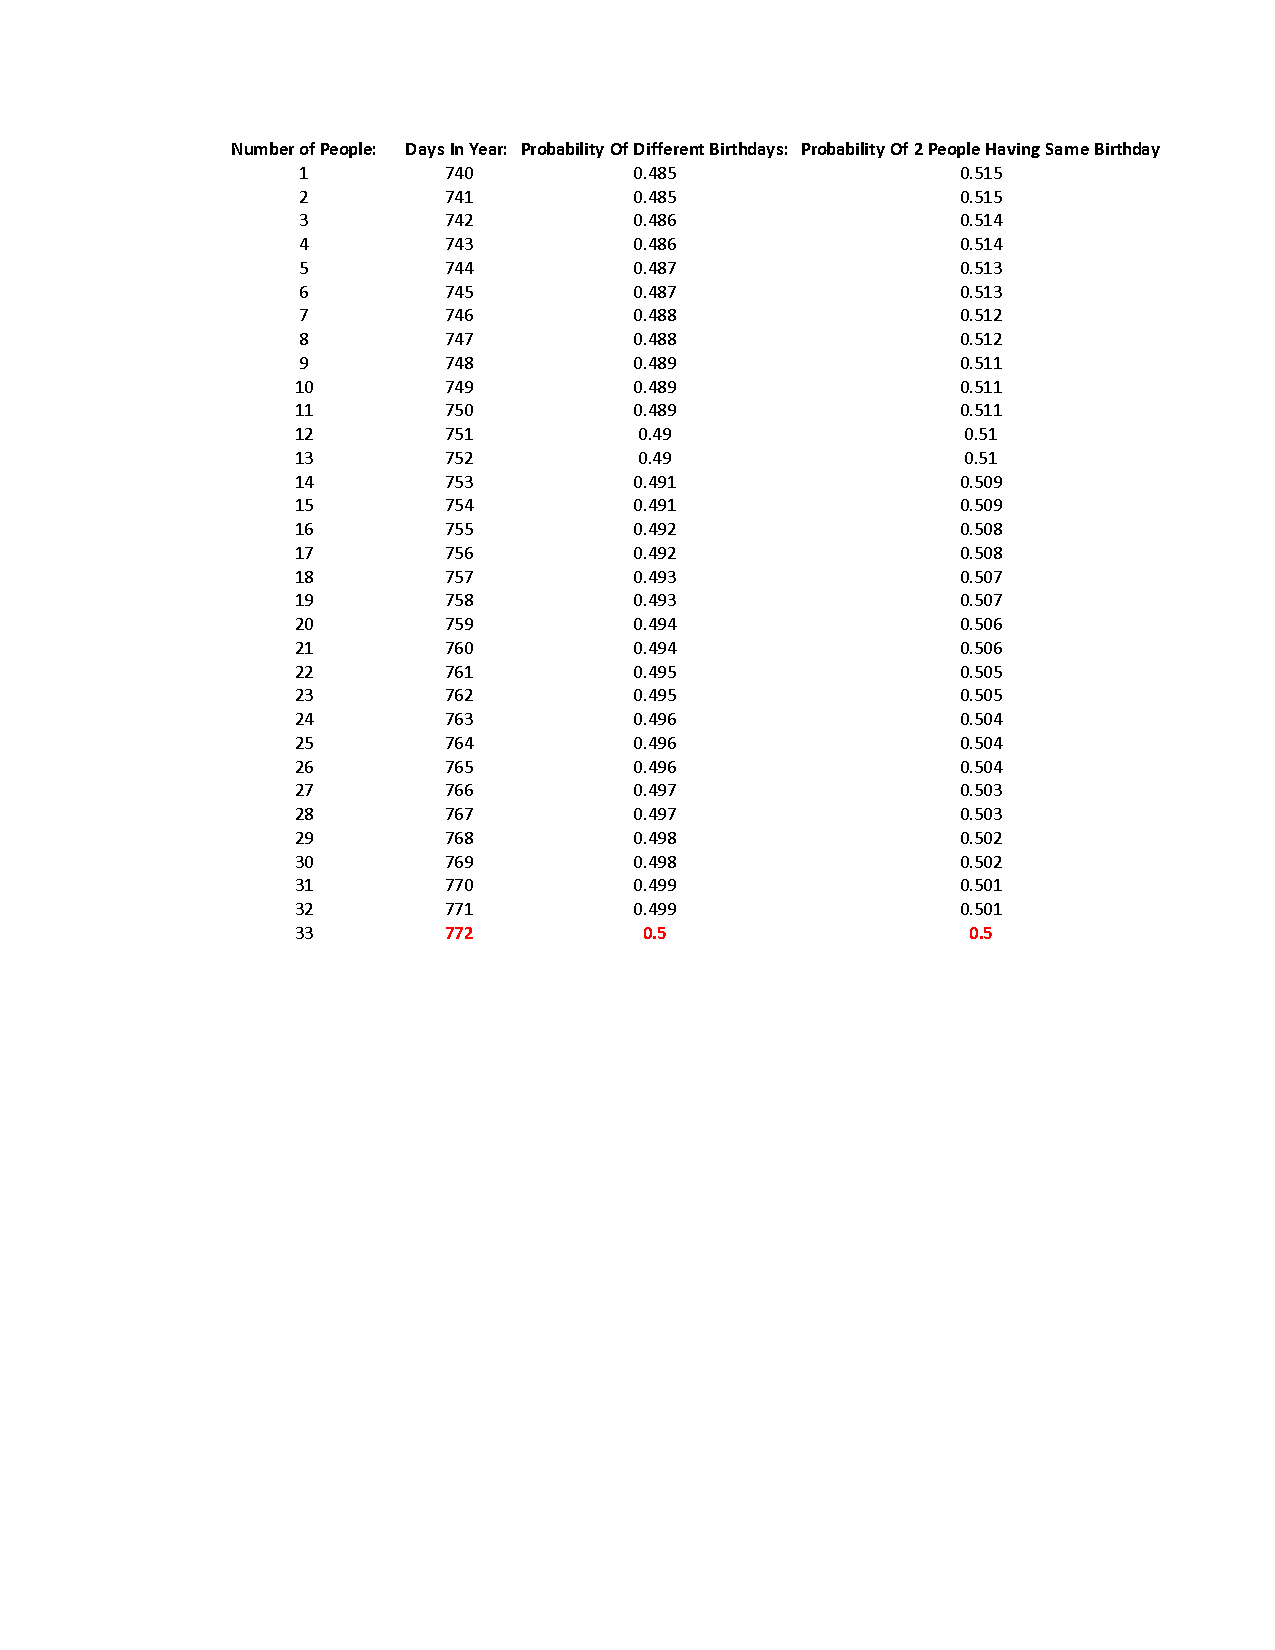
\includepdf[pages={-}, pagecommand={\thispagestyle{fancy}}, width=\paperwidth, offset=0 0]{./PDF/Birthday Problem.pdf} \clearpage
    \begin{Highlight}[Solution Continued]
        The values found for the number of people on the planet were calculated in column B. The number of days in the year were incremented in column C. The formula that was used to calculate the
        probability of different birthdays in column D was

        \begin{equation}
            \text{ROUND}(\text{PRODUCT}(((C3+1)-B\$3:B\$35)/C3),3)
        \end{equation}
        and then of course dragged down with new values for $C$. The formula that was used to calculate the probability of having the same birthday for two people in column E was

        \begin{equation}
            1-D3
        \end{equation}
        and dragged down to update the values for the entries in $D$. We can see that when this was done, we successfully recreated the formulae found in (1) and (2). After starting with 740 days,
        we were able to find the length of the year in days. The length of planet Probby was then found to be

        \begin{equation}
            \text{\textbf{772} days.}
        \end{equation}
    \end{Highlight}

    \begin{Highlight}[Python Solution]
        I decided to do this problem in Python as well even though it wasn't required for this assignment. Below is the code that I used to solve this problem.

    \begin{lstlisting}[style=stackoverflow, language=python]
    # BirthdayProblem - Calculates the number of days required for 2 people to having the same birthday at a desired probability
    # Input:
    #   numPeople - Number of people in data set
    #   desiredProbability - Desired probability of two people sharing the same birthday
    # Algorithm:
    #   * Set the break condition to 1
    #   * Set the number of days to be the number of people on the planet
    #   * Perform the following calculation until the probability is less than or equal to the desired
    #       * Increment the number of days
    #       * Calculate the probability of everyone having a different birthday for a set number of days
    #       * Calculate the probability of two people having the same birthday
    #   * Return the number of days
    # Output:
    #   days - Number of days required for two people amongst numPeople to have a desiredProbability chance of sharing the same birthday
    def BirthdayProblem(numPeople, desiredProbability):
        # Break condition probability
        sameProb = 1
        # Number of days
        days = numPeople
        # Repeat until sameProb <= desiredProbability
        while (sameProb > desiredProbability):
            # Increment the number of days
            days += 1
            # Set the different birthday prob to one
            diffProb = 1
            # Calculate the different birthday probability
            for i in range(1, numPeople + 1):
                iPeopleProb = ((days + 1) - i) / days
                diffProb *= iPeopleProb
            # Calculate the same birthday probability
            sameProb = round(1 - diffProb, 3)
        # Return number of days
        return days
    \end{lstlisting}
        Below is the output that I received from using the above function in the context of our problem.
    \begin{lstlisting}[style=stackoverflow]
    print(f"The number of days on this planet is: {BirthdayProblem(33, 0.50)} days.")

    taylor@Taylors-MacBook-Pro Code % python3 main.py
    
    The number of days on this planet is: 772 days.
    \end{lstlisting}
    \end{Highlight}
\end{problem}